\section{Smaud Myron}

\begin{center}
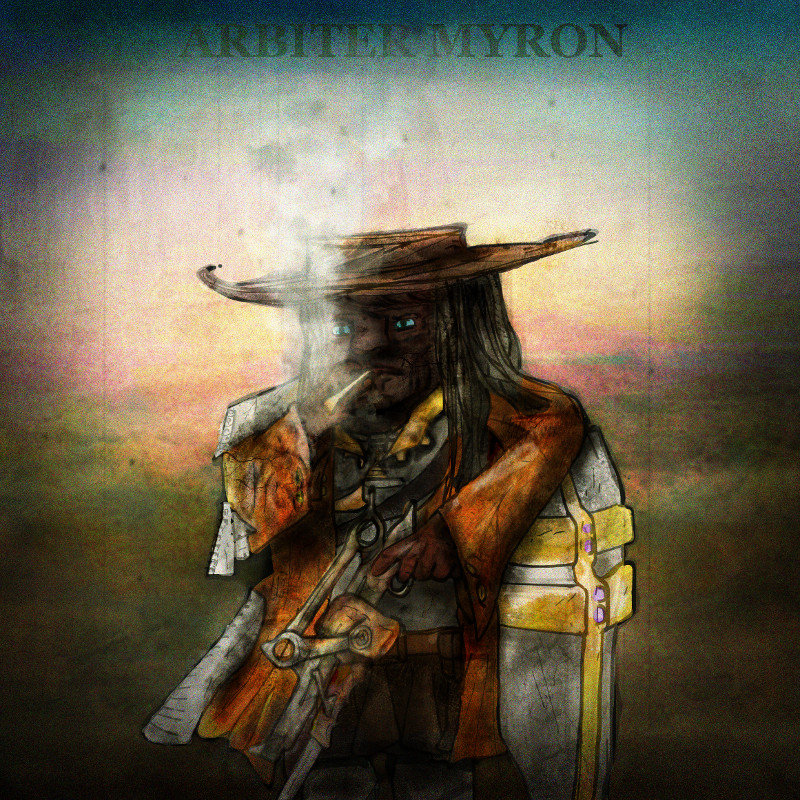
\includegraphics[width=80mm]{./content/img/myron1.png}
\begin{figure}[h]
\end{figure}
\end{center}

\subsection*{Details}

\noindent

Race: 	Gnome \\
Class: 	Arbiter \\
Age: 	80 \\
Status: Active

\subsubsection{Background}

Smaud Myron is a gnome Arbiter --- one of the Church's elite warrior-enforcers, trained in both martial combat and divine justice.  Older and more experienced than most of his companions, Myron carries the weight of a complicated past.  Decades ago, he was involved in the purge of the Book Burners, an act that placed him at odds with the very people he would later fight alongside.

Myron joined the party after a dramatic entrance involving a hot air balloon crash, bringing with him a level of tactical competence and martial skill that the group sorely needed.

\subsubsection{Personality and Traits}

Myron is serious, disciplined, and exceptionally skilled in combat.  He wields a gun with bayonet --- a combination weapon that allows him to fight at both range and in close quarters with devastating efficiency.  In battle, he is described as ``awesome'' with alarming frequency, sliding underneath enemies, slashing their underbellies, and generally being the most competent fighter the group has ever seen.

Outside of combat, Myron has a softer side.  He purchases personalised robes for the entire party, makes beef jerky as a comfort food, and bought a travel ping pong table that provided ``the happiest moment'' of Exme's life when she turned out to be a natural.  He expresses doubt about magical solutions (such as teleportation circles) but follows through with quiet professionalism.

\subsubsection{Relationships}

Myron and Exme have been involved in an ongoing ``will they, won't they'' relationship that Exme herself documented in a self-published novelette entitled ``Love Doesn't Have a Height Limit''.  Their connection deepened over the course of the Masuda campaign, with Myron caring deeply about Exme's safety and Exme becoming ``extremely jealous'' in the presence of other women near Myron.

Myron also developed a mutual respect with Riphard, the two bonding over their shared commitment to getting the job done, and he is known for his cooking which serves as a bonding mechanism with the wider group.

\subsubsection{Myron's Story}

Myron proved himself in the hunt for the Lord of Lightning --- a terrifying electric beast that had been killing balloon cows across the Masudan countryside.  While others prepared with ``a variety of levels of effectiveness, coolness and cowardice'', Myron slid underneath the creature, slashing and blasting its underbelly, emerging unscathed while the beast tried and failed to land a hit on him.

During the castle infiltration to rescue the nobleman's son Romjiro, Myron threw the Emperor's daughter Julieto out of a window --- and then fell out himself, temporarily dying before being revived.  His pragmatic approach to impossible situations made him the group's most reliable asset in their darkest hours.

\clearpage
